\documentclass{beamer}

\title{Power Subsystem Technical Update}
\author{Troy Astorino \and Eddie Obropta \and Jimmy Clark \and Vladimir Eremin}
\date{April 9, 2013}
\institute[16.83 -- MIT]{Space Systems Design \\ Massachusetts Institute of
  Technology}

\usepackage{graphicx}
\usepackage{amsmath}

\usetheme{CambridgeUS}
\usecolortheme{beaver}
\setbeamertemplate{section in toc}[square]
%\setbeamercolor{section number projected}[bg=black, fg=red]
\setbeamertemplate{navigation symbols}{} % remove navigation symbols

\begin{document}

\begin{frame}
\maketitle
\end{frame}

\begin{frame}
  \frametitle{Outline}
  \tableofcontents
\end{frame}

\section{General Power Calculations}
\begin{frame}
  \frametitle{Power Needed from Solar Arrays}
  \[P_{sa} = \frac{\left(\frac{P_d T_d}{X_d} + \frac{P_e
        T_e}{X_e}\right)}{T_d}\]

  \begin{itemize}
    \item $P_{sa}$ - power collected by solar array during day
    \item $P_e$ - eclipse power requirements
    \item $P_d$ - day power requirements
    \item $T_d$ - day period
    \item $T_e$ - eclipse period
    \item $X_d$ - efficiency of path to individual loads during day
    \item $X_e$ - efficiency of path to individual loads during eclipse
  \end{itemize}
\end{frame}

\begin{frame}
  \frametitle{End of Life Power Density}
  \[P_{BOL} = P_o I_d \cos{\theta}\]
  \[P_{EOL} = P_{BOL} (1 - D)^L\]

  \begin{itemize}
    \item $P_{BOL}$ - beginning of life power density
    \item $P_o$ - solar cell power output per unit area
    \item $I_d$ - inherent degradation
    \item $\theta$ - sun incident angle
    \item $P_{EOL}$ - end of life power density
    \item $D$ - degradation per unit time
    \item $L$ - lifetime
  \end{itemize}
\end{frame}

\begin{frame}
  \frametitle{Solar Array Area and Battery Mass}
  \[A_{sa} = \frac{P_{sa}}{P_{EOL}}\]

  \begin{itemize}
    \item $A_{sa}$ - solar array area
    \item $P_{sa}$ - power collected by solar array during day
    \item $P_{EOL}$ - end of life power density
  \end{itemize}
\end{frame}

\begin{frame}
  \frametitle{Energy Collection through STK}
\end{frame}

\section{Holodeck}
\begin{frame}
  \frametitle{Two Options: Optical Communications and RF Communications}
  \begin{center}
    Using optical communications instead of RF communications changes
    duration and power usage for almost all modes.

    Will show more complete calculations for RF communications, rough
    calculations for optical communications.
  \end{center}
\end{frame}

\section{DeMi}

\begin{frame}
	\frametitle{Requirements}

		
	\[ E_{req,orb} = \sum_\text{modes}{\sum_\text{systems}{T_{mode}P_{sys,mode}}} \]
	
	\[  P_{req,avg} = \frac{E_{req,orb}}{T_{orbit}} \]
	
	\[ E_{req,batt} = P_{req,avg} \times T_e\]
	
	(TBD)
	
\end{frame}

\begin{frame}
	\frametitle{Capacity}
	\begin{columns}
	\begin{column}{0.5\textwidth}
	$ \displaystyle E_{panels,orb} = \int_{orbit}{P_{panel}\cos\theta \ dt } $
	\newline
	\newline
	$ \displaystyle P_{panels,avg} = \frac{E_{panels,orb}}{T_{orbit}} \approx 6.5 W \ \text{(TBR w/ STK)}$
	
	\begin{center}
	Check: $P_{panels,avg} \geq P_{req,avg}$ (almost), $E_{batt} \geq E_{req,batt}$	(OK)
	\end{center}
	
	\end{column}
	
	\begin{column}{0.5\textwidth}
	
	\begin{figure}%
	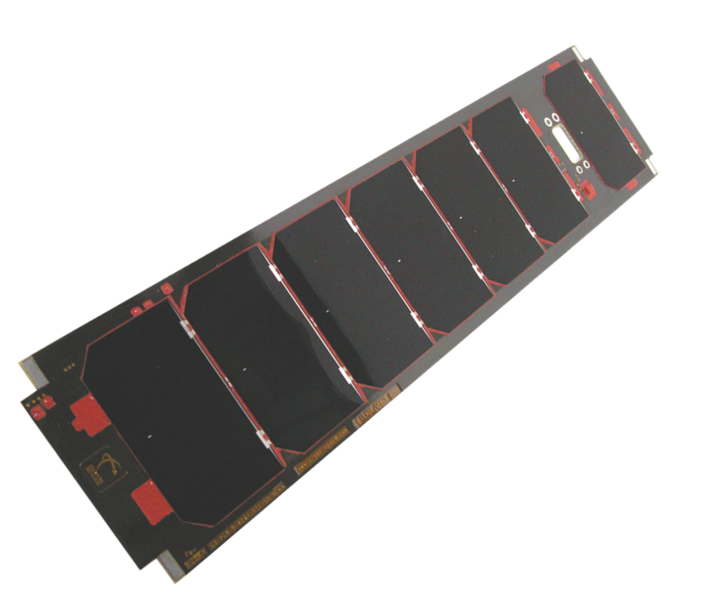
\includegraphics[width=\columnwidth]{Panel}%
	\caption{Clyde Space 3U Cubesat solar panel}%
	\label{}%
	\end{figure}
	\end{column}
	
	\end{columns}
	
\end{frame}

\end{document}
